\documentclass{ximera}
%\documentclass[handout,space,nooutcomes]{ximera}

\title{Paying off Debt, Part 2}

\begin{document}
\begin{abstract}
Here we continue to investigate where your payments go when you pay off debt.
\end{abstract}
\maketitle


\begin{question}
Suppose you borrow $\$P$ and agree to pay it back in equal annual
payments over $n$ years, with an annual interest rate of $r$, compounded annually.  
Call the annual payment $x$, and write an equation that must be true if
the payment amount is correct.  

\begin{hint}
Use your table from last week's class, showing the interest, payment, and remaining
principal at the end of years $1, 2, 3, \dots$, and try to see
patterns in the table.  It helps to collect factors of $(1+r)$.
\end{hint} 
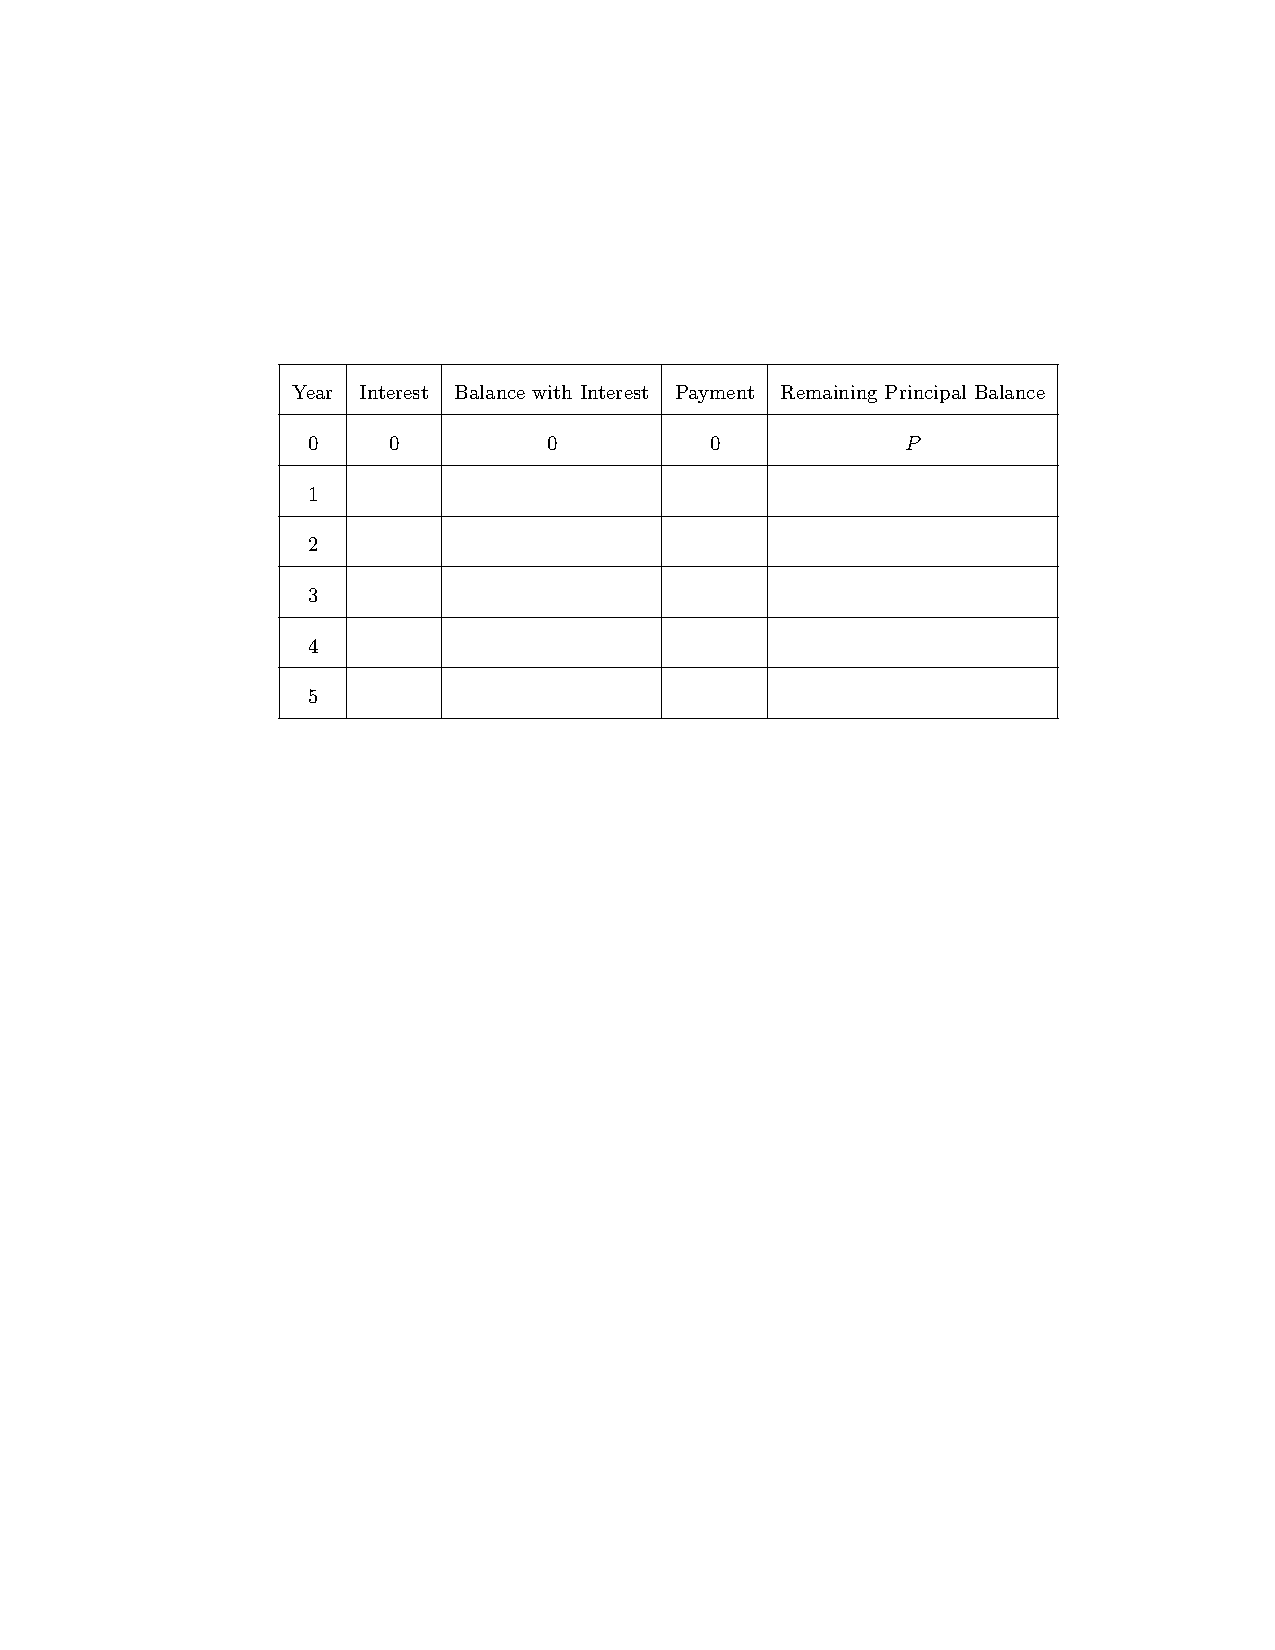
\includegraphics{payingOffDebtTableGraphic2.pdf}

\begin{freeResponse}
\end{freeResponse}
\end{question}


\begin{question}
Some students notice that the equation above includes a geometric series.  Write that geometric series here.
\begin{freeResponse}
\end{freeResponse}
\end{question}

\begin{question}
How do you know this is a series?  How do you know this is a geometric series?   
\begin{freeResponse}
\end{freeResponse}
\end{question}

\begin{question}
Find a closed-form expression for the sum of the geometric series.  
\begin{freeResponse}
\end{freeResponse}
\end{question}

%\begin{question}
%Call the geometric series $S$, and note that if you multiply $S$ by $r$, the ``common ratio,'' you get another geometric series with many of the same terms.  Use these observations to find the sum of the series.   
%\begin{freeResponse}
%\end{freeResponse}
%\end{question}


\begin{question}
Use the closed-form expression for the sum of the geometric series to solve your equation for $x$, the annual payment.   
\begin{freeResponse}
\end{freeResponse}
\end{question}

\begin{question}
What about monthly payments?  In other words, suppose you borrow $\$P$ and agree to pay it back in equal monthly
payments over $n$ years, with an annual interest rate of $r$, compounded monthly.  
Write a formula for the monthly payment.  
\begin{freeResponse}
\end{freeResponse}
\end{question}


\begin{question}
Now suppose that you buy a house with a $\$120,000$ mortgage, to be
paid back in equal monthly payments over $30$ years.  If the interest
rate is $6\%$, compounded monthly, what is your monthly payment?
\begin{freeResponse}
\end{freeResponse}
\end{question}

\break

\begin{question}
In the mortgage question, how much interest and how much principal
would you pay in the first month? Why? What about the second month? What about the final month?
\begin{freeResponse}
\end{freeResponse}
\end{question}

\begin{question}
In the mortgage question, how much interest would you pay in total
over the $30$ years?
\begin{freeResponse}
\end{freeResponse}
\end{question}

\begin{question}
Finding an equal monthly payment for paying off a debt is a foundational problem in financial mathematics.  
How might this problem change for more complicated financial transactions?  Consider the perspectives of 
borrowers, lenders, bankers, investors, etc.  
\begin{freeResponse}
\end{freeResponse}
\end{question}



\end{document}
